% Dokumentklassen s�ttes til memoir.
% Manual: http://ctan.org/tex-archive/macros/latex/contrib/memoir/memman.pdf
\documentclass[a4paper,oneside,article]{memoir}

\usepackage{pgf}
\usepackage{tikz}
\usepackage{pgfplots}
\usetikzlibrary{arrows,automata}
\usepackage{verbatim}
 
% Danske udtryk (fx figur og tabel) samt dansk orddeling og fonte med
% danske tegn. Hvis LaTeX brokker sig over �, � og � skal du udskifte
% "utf8" med "latin1" eller "applemac". 
\usepackage{inputenc}
\usepackage[danish]{babel}
\usepackage[T1]{fontenc}
 
% Matematisk udtryk, fede symboler, theoremer og fancy ting (fx k�debr�ker)
\usepackage{amsmath,amssymb}
\usepackage{bm}
\usepackage{amsthm}
%\usepackage{mathtools}
 
% Kodelisting. Husk at l�se manualen hvis du vil lave fancy ting.
% Manual: http://mirror.ctan.org/macros/latex/contrib/listings/listings.pdf
\usepackage{listings}
 
% Fancy ting med enheder og datatabeller. L�s manualen til pakken
% Manual: http://www.ctan.org/tex-archive/macros/latex/contrib/siunitx/siunitx.pdf
%\usepackage{siunitx}

% Inds�ttelse af grafik.
\usepackage{graphicx}
\usepackage{float}
\usepackage{caption}
\usepackage{subcaption}
 
% Reaktionsskemaer. L�s manualen for at se eksempler.
% Manual: http://www.ctan.org/tex-archive/macros/latex/contrib/mhchem/mhchem.pdf
%\usepackage[version=3]{mhchem}
%\usepackage[noend]{algpseudocode}
%\usepackage{algorithm}

\usepackage{xcolor,colortbl}

\usepackage{listings}

\definecolor{javared}{rgb}{0.6,0,0} % for strings
\definecolor{javagreen}{rgb}{0.25,0.5,0.35} % comments
\definecolor{javapurple}{rgb}{0.5,0,0.35} % keywords
\definecolor{javadocblue}{rgb}{0.25,0.35,0.75} % javadoc

\lstset{language=Java,
basicstyle=\small, %\ttfamily,
keywordstyle=\color{javapurple}\bfseries,
stringstyle=\color{javared},
commentstyle=\color{javagreen},
morecomment=[s][\color{javadocblue}]{/**}{*/},
numbers=left,
numberstyle=\tiny\color{black},
stepnumber=1,
numbersep=10pt,
tabsize=4,
showspaces=false,
showstringspaces=false}

\newcommand{\notimplies}{%
  \mathrel{{\ooalign{\hidewidth$\not\phantom{=}$\hidewidth\cr$\implies$}}}}

\begin{document}
    \title{Client-centric consistency - Disposition}
    \author{Lukas Peter J�rgensen, 201206057, DA4
            }
    \maketitle
    
    \chapter{Introduction}
	\begin{figure}[H]
		\centering
		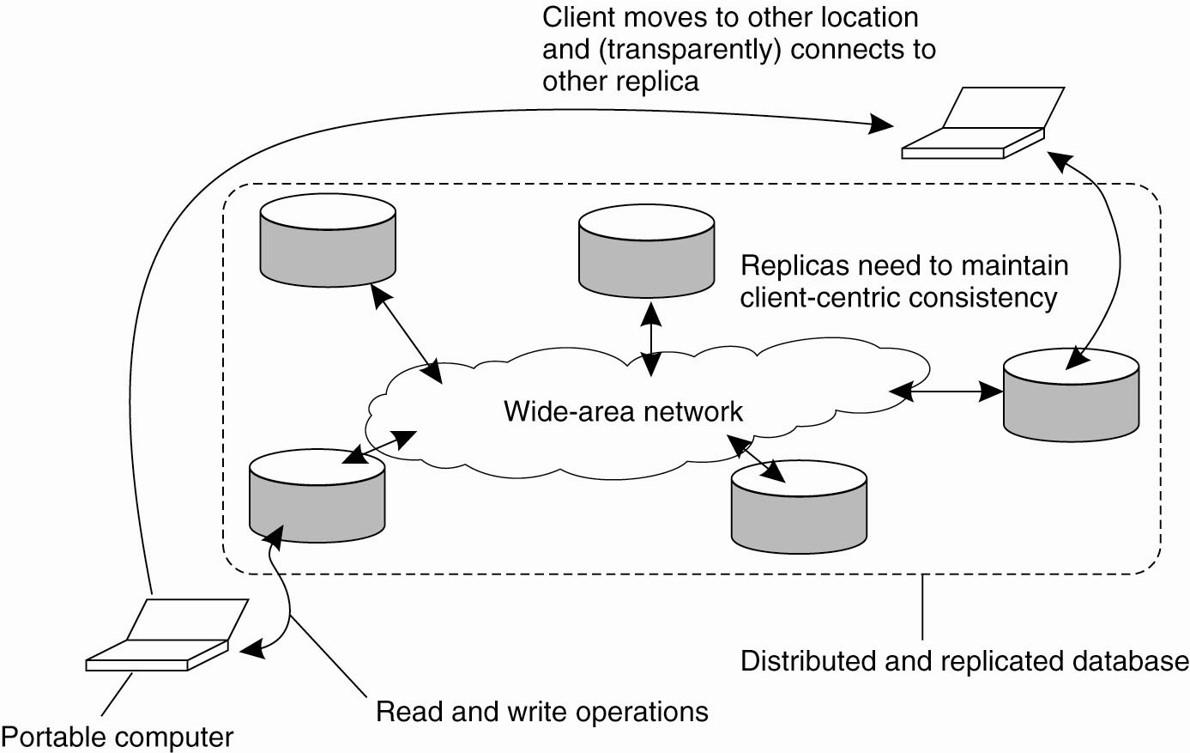
\includegraphics[width=\textwidth]{Media/ClientCentInt.jpg}
	\end{figure}
	I want the database to be consistent to me, that is I only care that the entries I edited in A, are in B the way I left them in A.\\
	\textbf{Monotonic reads}\\
	If a process reads the value of a data item $x$, any successive read operation on $x$ by that process will always return that same or a more recent value.
	\begin{figure}[H]
		\centering
		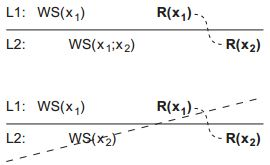
\includegraphics{Media/MonoReads.jpg}
	\end{figure}
	\textbf{Monotonic writes}\\
	A write operation on a data item $x$ is completed before any successive write operation on $x$ by the same process.
	\begin{figure}[H]
		\centering
		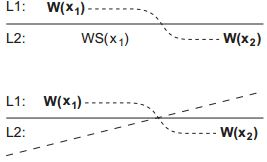
\includegraphics{Media/MonoWrites.jpg}
	\end{figure}
	\textbf{Read your writes}\\
	The effect of a write operation by a process on data item $x$, will always be seen by a successive read operation on $x$ by the same process.
	\begin{figure}[H]
		\centering
		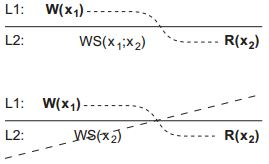
\includegraphics{Media/ReadUrWrites.jpg}
	\end{figure}
	\textbf{Writes follow reads}\\
	A write operation by a process on a data item $x$ following a previous read operation on $x$ by the same process, is guaranteed to take place on the same or a more recent value of $x$ that was read.
	\begin{figure}[H]
		\centering
		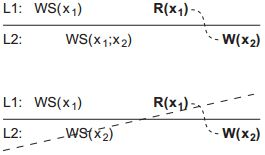
\includegraphics{Media/WritesFolReads.jpg}
	\end{figure}
	
    
\end{document}